\documentclass[10pt,a4paper]{article}
%\usepackage[utf8]{inputenc}
\usepackage[margin=0.5in]{geometry}
\usepackage{graphicx}
\author{
  Drew, Keith\\
  \texttt{keithd@vandals.uidaho.edu}
  \and
  Jaszkowiak, Tyler\\
  \texttt{jasz7989@vandals.uidaho.edu}
  \and
  Pearhill, Gabe\\
  \texttt{pear9915@vandals.uidaho.edu}
  \and
  Klingenberg, David\\
  \texttt{bigwookie@gmail.com}
  \and 
  Fuhrman, Wayne\\
  \texttt{fuhr0438@vandals.uidaho.edu}
  \and
  Goes, Chris\\
  \texttt{goes8945@vandals.uidaho.edu}
}
\title{Diagram Assembly Document}
\begin{document}
\maketitle
\section{Dictionary}
\begin{itemize}
\item Board: The game board, this holds nearly all visual information about the game and state. The class holds random event flags, which will become more specific, that indicate global events.
\item Province: A province is a group of hexes that are related by controlling faction. Essentially like the United States of Hexes. 
\item Hex: A discrete location on the board. Hexes are represented by a unique ID, terrain, and a stack of units that can be empty.
\item Stack: A collection of units and characters, bound by the rules of the game. Ie, 0 or more characters, and 0-2 units. Also, special considerations for movement phase, flying units, and monsters.
\item Vortex: A vortex is a moveable unit, from the system's point of view. A character can control vortices under certain conditions. Otherwise movement, creation, and destruction of vortices is automated.
\item Diplomacy: An object defining the relationship between players and neutral entities.
\item Player: The human player. This object contains information about the players armies, diplomatic relations, race, and victory points.
\item Army: This object is responsible for conveniently managing the units of each individual diplomatic entity.
\item Spells: An object that contains the stats and effects of each castable spell.
\end{itemize}

\pagebreak
\section{Team A Class Diagram}
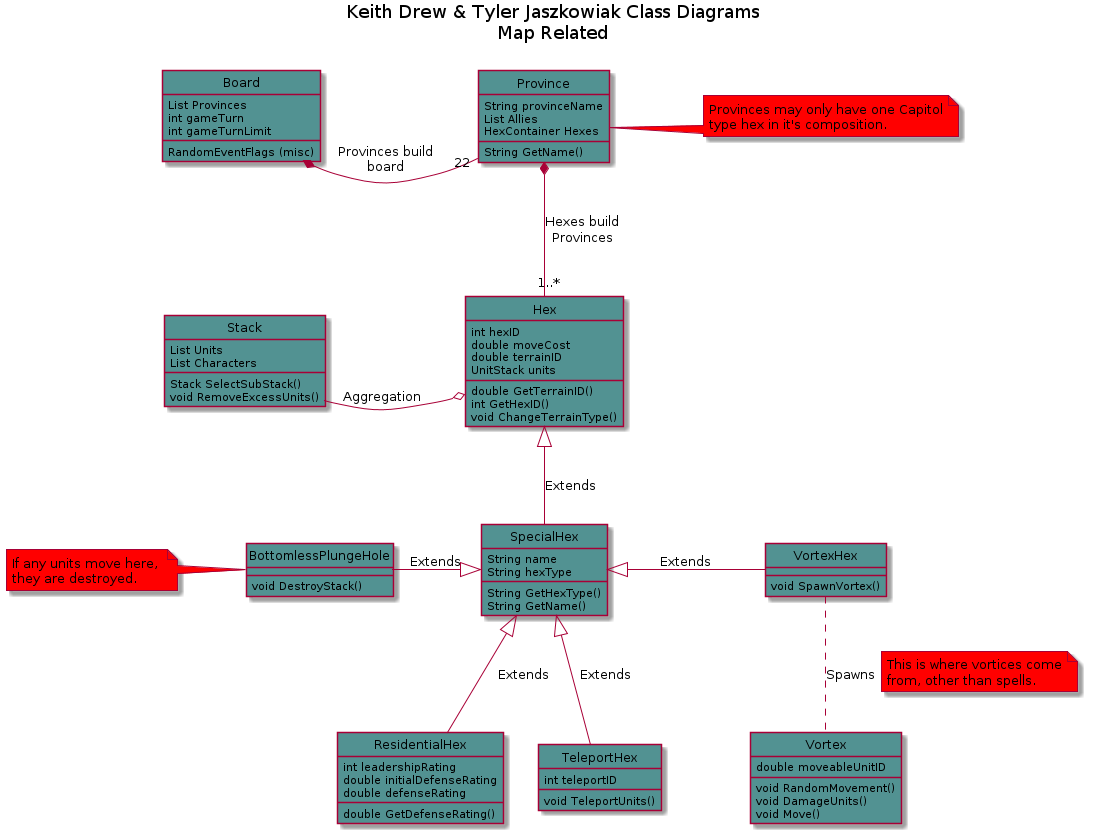
\includegraphics[width=\textwidth]{classD}

\section{PlantUML Source}
\begin{verbatim}



\end{verbatim}


\section{Detail Diagrams}

\subsection{Blah Detail}

Picture here!
\begin{verbatim}

Plant UML here!

\end{verbatim}

\end{document}
